\documentclass{beamer}
\usepackage[utf8]{inputenc}
\usepackage{graphicx}
\usetheme{Warsaw}
\usecolortheme{seahorse}

\title{Cancer Analysis Workflow Sprint Review}
\institute{SciLifeLab}
\date{14th November 2016 }
\begin{document}
\frame{\titlepage}
			  
\begin{frame}
\frametitle{Cancer Analysis Workflow Sprint Review}
\begin{block}{What happened in the last month?}
    \begin{itemize}
	\item Features in release v0.9
        \item Refactoring code
	\item DREAM challenge results
	\item Next steps
    \end{itemize}
    Although focus was on processing the DREAM challenge data, many new features were added, bugs fixed.
\end{block}
\end{frame}

\begin{frame}
\frametitle{Features in release v0.9}
This release is capable to process tumour/normal pairs starting from raw FASTQ files, or from preprocessed BAM files.
	\begin{block}{Features we are expected to work}
            \begin{itemize}
                \item Preprocessing (Alignment, Merging... all the steps to get a base-recalibrated BAM)
                \item SNP and indel callers: MuTect1 and Strelka working
                \item SV caller: Manta
            \end{itemize}
	\end{block}
        \begin{block}{Features for better user experience}
	    \begin{itemize}
		\item Start from realignment: we have to realign BAMs together
		\item One can chose different targets (Manta,MuTect1,... and their combination)
		\item Restart only from the finished preprocessing step
                \item More documentation
	    \end{itemize}
        \end{block}
\end{frame}

\begin{frame}
\frametitle{DREAM challenge synthetic sets}
	\begin{block}{First set of somatic call challenges}
            Using pre-processed BAM files provided by TCGA compare variant callers for better somatic call results.

            Published results after several steps of optimizations

            Our results are listed as the very first approach

	    \begin{itemize}
		\item S1: 3537 somatic SNVs, 100\% tumour, few indels and SVs
		\item S2: 4332 somatic SNVs, 80\% tumour, some indels and SVs
		\item S3: 7903 somatic SNVs, 33\% tumour, 20\% different subclone, many indels and SVs
	    \end{itemize}
	\end{block}
\end{frame}

\begin{frame}
\frametitle{Getting consensus calls}
    \begin{block}{SNPs are called only if both MuTect1 and Strelka gives a call}
        \begin{itemize}
            \item Expected to have a SOMATIC info flag (both caller classified the SNP as a somatic one)
            \item Expected to have a PASS filter by both callers (both caller was confident in the call)
        \end{itemize}
        Recall and precision was calculated by the python script provided by the ICGC-TCGA DREAM group
        \begin{itemize}
            \item $ recall = \frac{TP}{TP + FN}$
            \item $ precision = 1 - \frac{FP}{(TP + FP)}$
            \item $ F_{score} = 2 \times \frac{precision \times recall}{precision + recall}$
        \end{itemize}
    \end{block}
\end{frame}

\begin{frame}
\frametitle{DREAM challenge - SNPs}
\center { 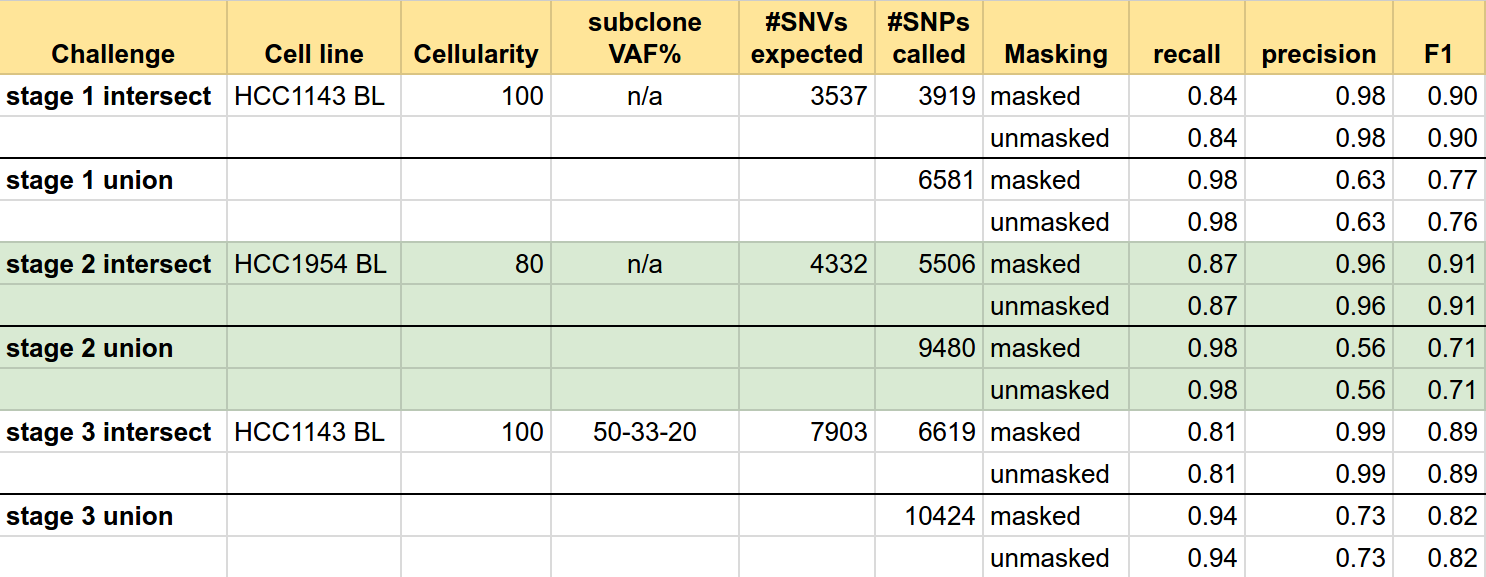
\includegraphics[width=1\linewidth]{DREAM_SNPs.png} }
\end{frame}

\begin{frame}
\frametitle{DREAM challenge - SNPs stage 1}
\center { 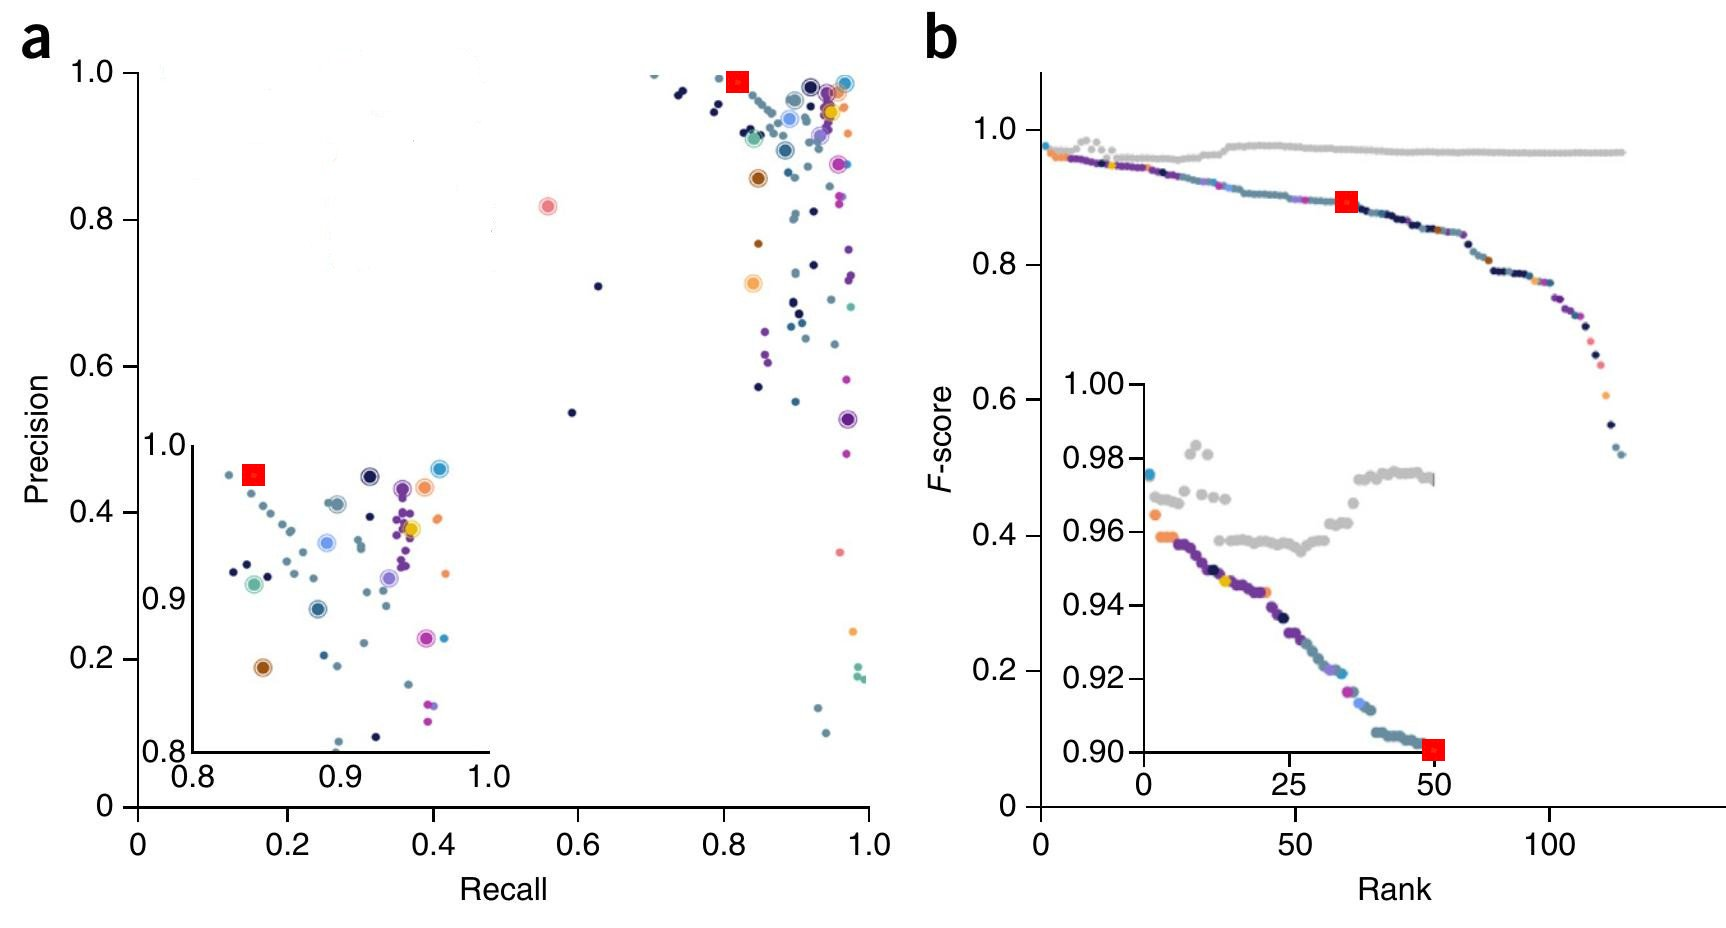
\includegraphics[width=1\linewidth]{S1.jpg} }
\end{frame}

\begin{frame}
\frametitle{DREAM challenge - SNPs stage 2}
\center { 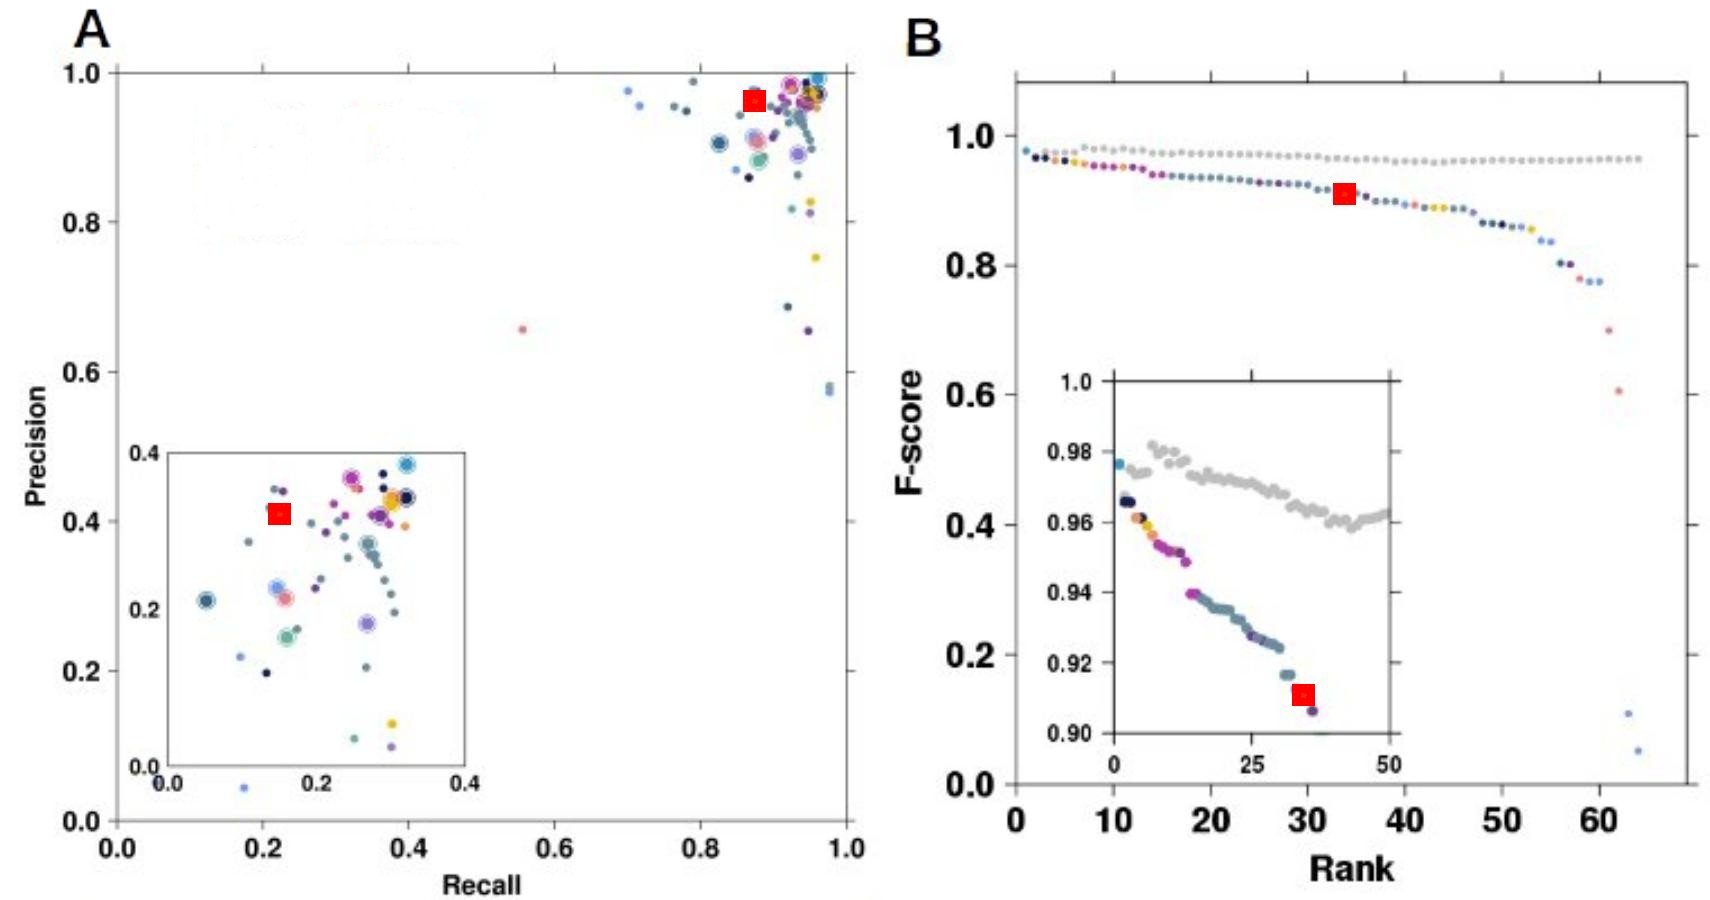
\includegraphics[width=1\linewidth]{S2.jpg} }
\end{frame}

\begin{frame}
\frametitle{DREAM challenge - SNPs stage 3}
\center { 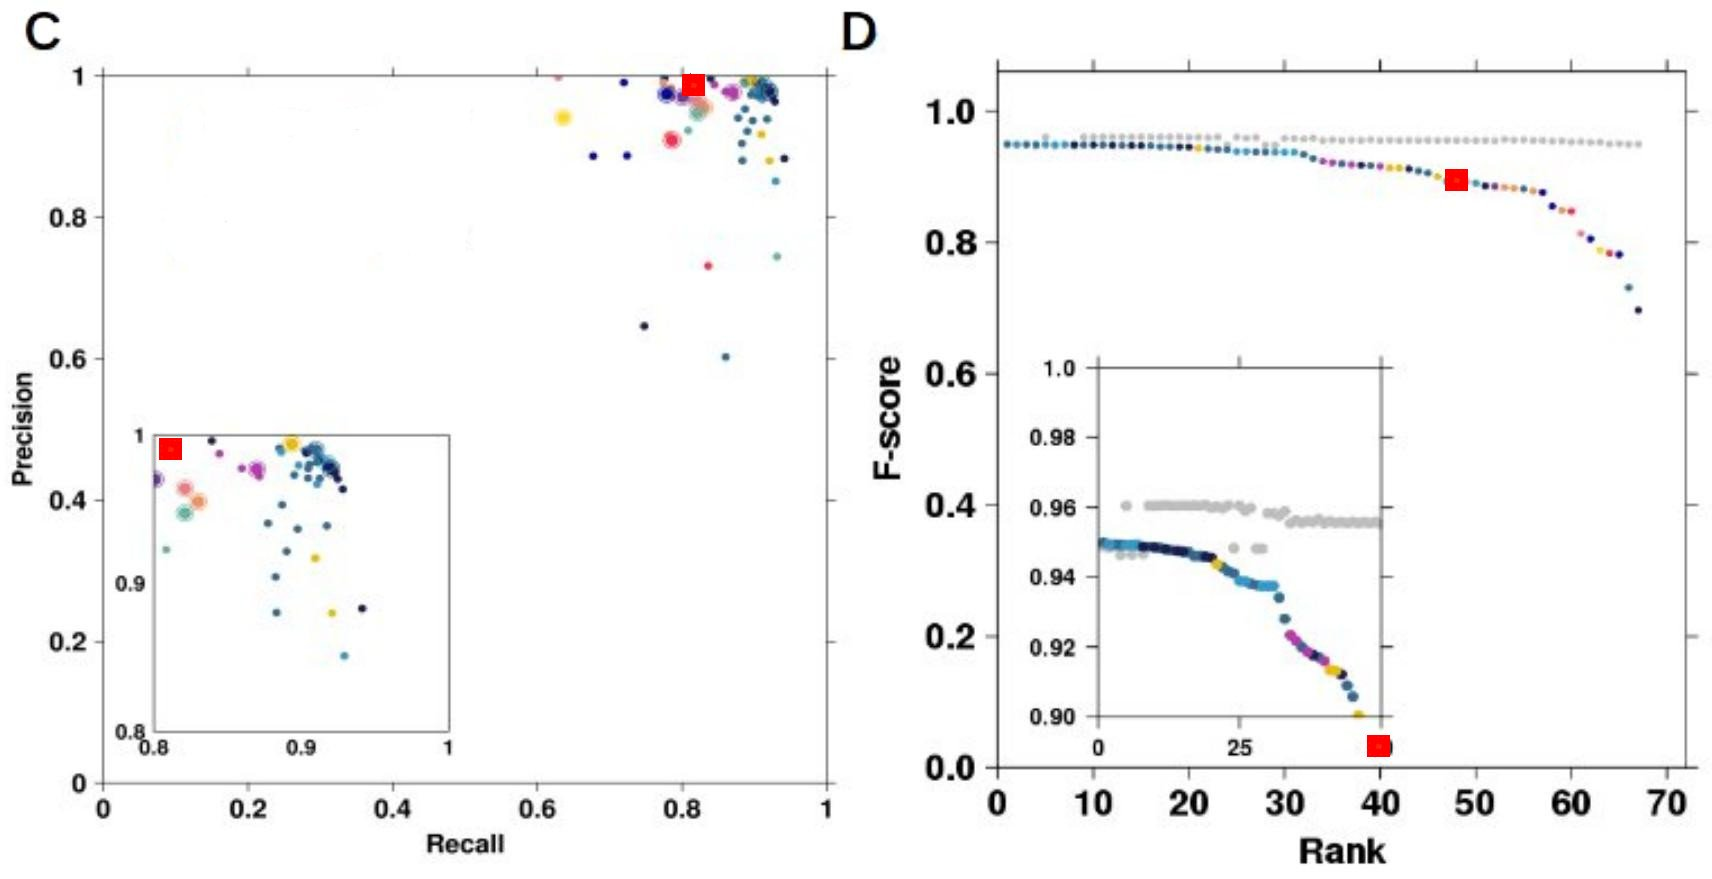
\includegraphics[width=1\linewidth]{S3.jpg} }
\end{frame}

\begin{frame}
\frametitle{DREAM challenge - indels}
\center { 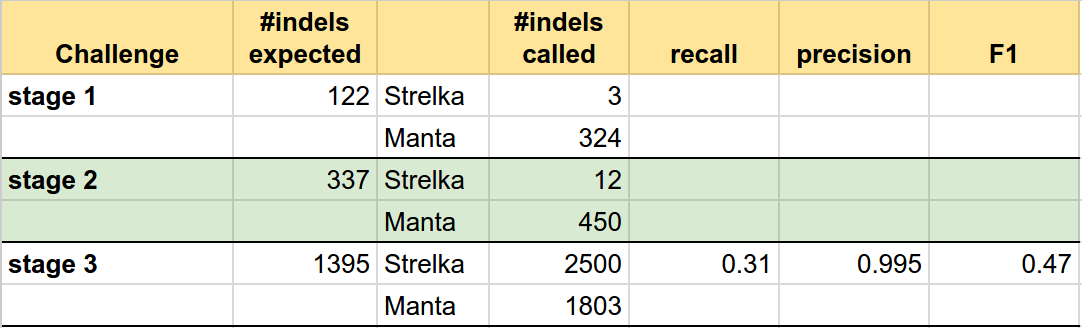
\includegraphics[width=1\linewidth]{DREAM_indels.png} }
\end{frame}

\begin{frame}
\frametitle{DREAM challenge - SVs}
\center { 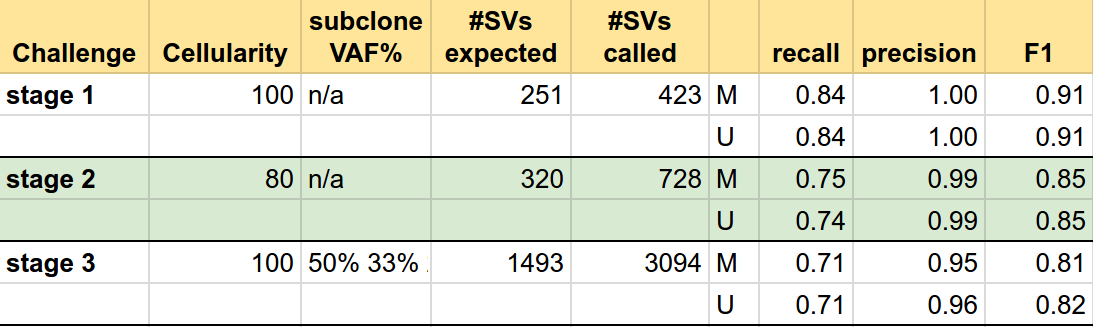
\includegraphics[width=1\linewidth]{DREAM_SVs.png} }
\end{frame}

\begin{frame}
\frametitle{Purity and clonality tests in the DREAM challenge}
\center { 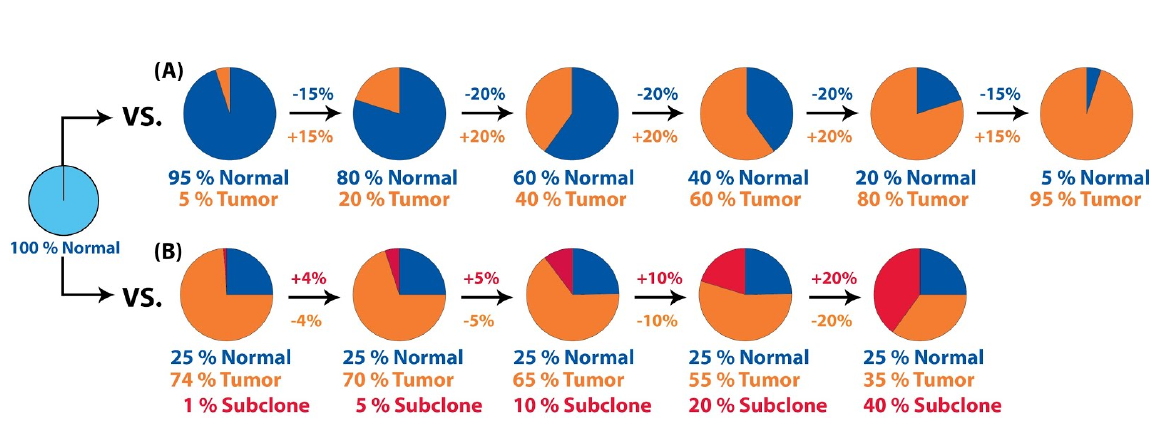
\includegraphics[width=1\linewidth]{DREAM_Clones.png} }
\end{frame}

\begin{frame}
\frametitle{Purity HCC1143}
\center { 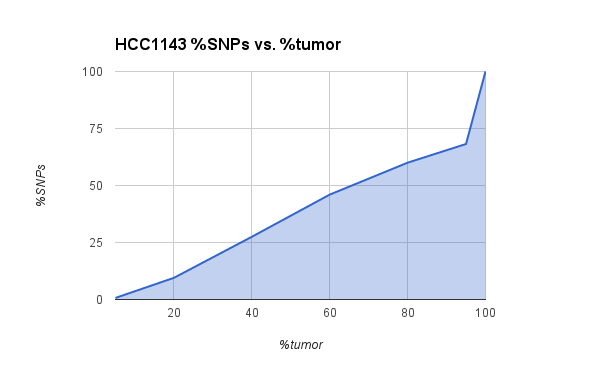
\includegraphics[width=1\linewidth]{HCC1143_purity.png} }
\end{frame}

\begin{frame}
\frametitle{Purity HCC1954}
\center { 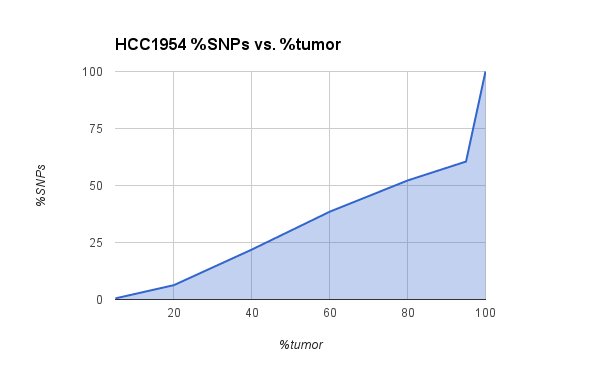
\includegraphics[width=1\linewidth]{HCC1954_purity.png} }
\end{frame}

\begin{frame}
\frametitle{Conclusions about purity}
    \begin{itemize}
        \item We are getting something we were expected to get
        \item No idea why we are loosing SNVs so quickly
        \item Sensitivity: at 20\% tumour content we can see almost nothing (contradicts to challenge S3)
        \item More/better tests are needed
        \item Will be worth to compare results from other software (i.e. ASCAT) 
    \end{itemize}
\end{frame}

\begin{frame}
\frametitle{Purity and clonality tests in the DREAM challenge}
\center { 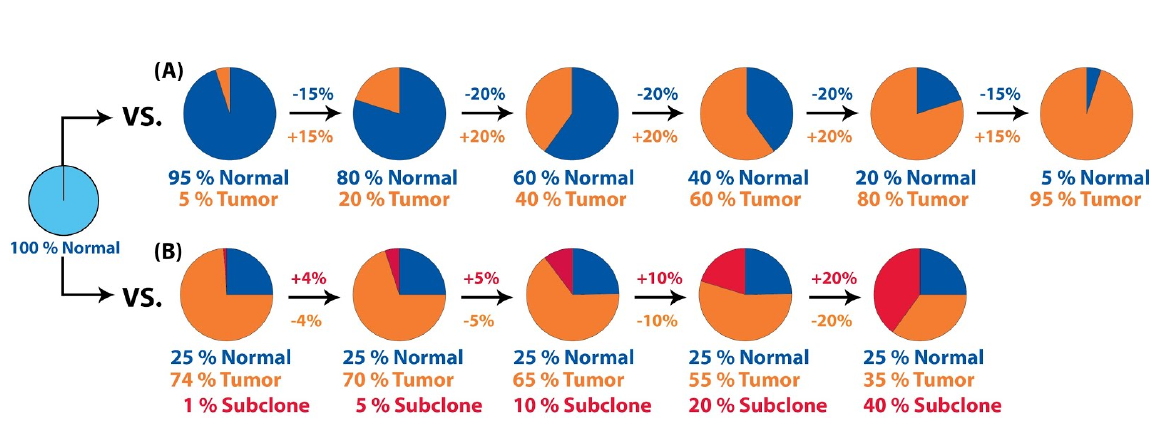
\includegraphics[width=1\linewidth]{DREAM_Clones.png} }
\end{frame}

\begin{frame}
\frametitle{Clonality tests HCC1143}
\center { 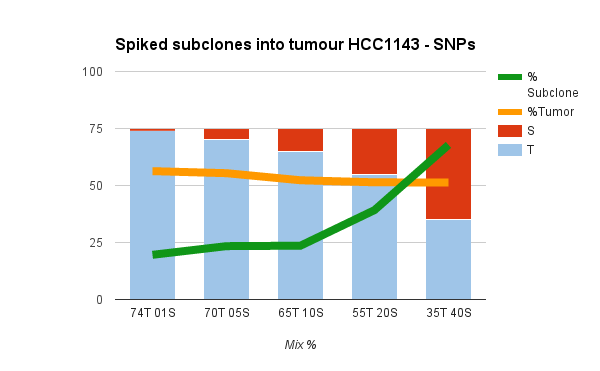
\includegraphics[width=1\linewidth]{HCC1143_subclones.png} }
\end{frame}

\begin{frame}
\frametitle{Clonality tests HCC1954}
\center { 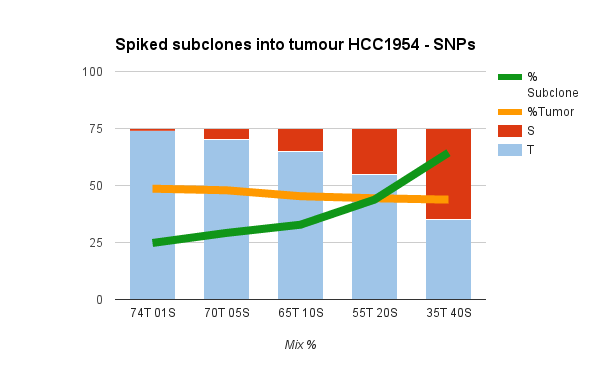
\includegraphics[width=1\linewidth]{HCC1954_subclones.png} }
\end{frame}

\begin{frame}
\frametitle{Conclusions about clonality}
    \begin{itemize}
        \item Not clear why we have high recall for subclones
        \item Seems we can have somatic calls at low tumour concentration
        \item Have no tools to distinguish clones (i.e. when adding relapse samples)
    \end{itemize}
\end{frame}

\begin{frame}
\frametitle{Towards version 1.0}
    \begin{itemize}
        \item Refine SNV call recall {\it and} precision (get higher F values)
        \item Refine indels (look around for an alternative caller and improve selection)
        \item Add ASCAT 
        \item Provide a merged VCF for ranking
    \end{itemize}
\end{frame}

\begin{frame}
\frametitle{Towards version 2.0}
    \begin{itemize}
        \item Add more test cases (sensitive data: we have to fill out papers)
        \item Add CNVs (got relatively little focus)
        \item Persuade users to use the workflow: to surface bugs and features 
        \item Refactoring: must happen continuously
    \end{itemize} 
\end{frame}

\begin{frame}
\frametitle{Longer term plans}
    \begin{itemize}
        \item Variant annotation
        \item Variant scoring/ranking
        \item Program cancer interface in Scout/Puzzle/New software
        \item Flexible choice in how to treat several variant callers (intersect, overlap, scoring etc)
        \item Set up CAW on Clinical Genomics’ hardware
        \item Switch to GrCh38
        \item Exome/custom capture support and QC
        \item Integrate with RNA seq 
    \end{itemize} 
\end{frame}


\begin{frame}
\frametitle{Final remarks}
    \begin{itemize}
	\item The workflow is robust - providing the underlying infrastructure works
            \begin{itemize} \item We have no information about Bianca right now \end{itemize}
	\item Have to be more user-friendly
            \begin{itemize} \item Malin as primary test user on real data \end{itemize}
            \begin{itemize} \item Teresita already used the workflow, and found some trivial inconsistencies \end{itemize}
            \begin{itemize} \item Command-line interface is going to be stable\end{itemize}
        \item Nextflow looks like a good choice, we have an active user/developer community
        \item I am actually surprised that the DREAM challenge results are OK - thanks for the input from Oslo!
    \end{itemize}
\end{frame}

\begin{frame}
\frametitle{TODO}
\begin{itemize}
	\item Fix the recall/precision rate values reported for Manta SVs
	\item Report SNPs/indels/SVs in a separate set of files
	\item Report all the four options for SNPs (MuTect1 only, Strelka only, union, intersection)
	\item Prioritize recall (sensitivity) 
	\item Check Manta indel reports/possible optimization
	\item Control-FREEC / Canvas validation by Malin?
\end{itemize}
\end{frame}

\end{document}
